%\renewcommand{\theequation}{\theenumi}
%\begin{enumerate}[label=\thesubsection.\arabic*.,ref=\thesubsection.\theenumi]
%%\begin{enumerate}[label=\arabic*.,ref=\thesection.\theenumi]
%\numberwithin{equation}{enumi}


\item Construct a quadrilateral $ABCD$ such that $AB=5, \angle A = 50\degree, AC = 4, BD = 5$ and $AD = 6$.
\\
\solution 
\begin{enumerate}
    \item Given point $\vec{P} = \myvec{-4\\3}$ and slope $m = \frac{1}{2}$.
    The direction vector is $\vec{m} = \myvec{2\\1}$.  
    Hence, the normal vector
    \begin{align}
    \label{linform/2/14/eq:line_norm_dir}
    \vec{n} &= \myvec{0&-1\\1&0}\vec{m} 
    \\
    &= \myvec{-1\\2}
    \end{align}
    The equation of the line in terms of the normal vector is then obtained as
    \begin{align}
    \label{linform/2/14/eq:line_norm_vec}
    \vec{n}^T\brak{\vec{x}-\vec{A}} &= 0
    \\
    \implies \myvec{-1 & 2} \vec{x} &= 10
    \end{align}
    See Fig.     \ref{linform/2/14/Plot of Line $AB$ (Part-1)}
    \begin{figure}[ht]
    \centering
    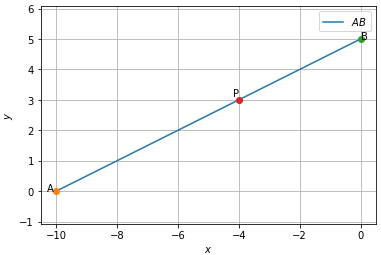
\includegraphics[width=\columnwidth]{solutions/su2021/2/14/Line_Plot_Part1.PNG}
    \caption{Plot of Line $AB$ (Part-1)}
    \label{linform/2/14/Plot of Line $AB$ (Part-1)}
    \end{figure}
    \item Given point $\vec{P} = \myvec{2\\2\sqrt{3}}$.From the given information we have, $\tan75\degree =m = \frac{\sqrt{3}+1}{\sqrt{3}-1}$.
    The direction vector is $\vec{m} = \myvec{1\\\tan75\degree}$.  
    Hence, the normal vector
    \begin{align}
    \label{linform/2/14/eq:line_norm_dir2}
    \vec{n} &= \myvec{0&-1\\1&0}\vec{m} 
    \\
    &= \myvec{-\tan75\degree\\1}
    \end{align}
    The equation of the line in terms of the normal vector is then obtained as
    \begin{align}
    \label{linform/2/14/eq:line_norm_vec2}
    \vec{n}^T\brak{\vec{x}-\vec{A}} &= 0
    \\
    \implies \myvec{-\sqrt{3}+1 &\sqrt{3}-1}  \vec{x} &= -4\brak{\sqrt{3}-1}
    \end{align}
    See Fig. \ref{linform/2/14/Plot of Line $AB$ (Part-2)}

    \begin{figure}[ht]
    \centering
    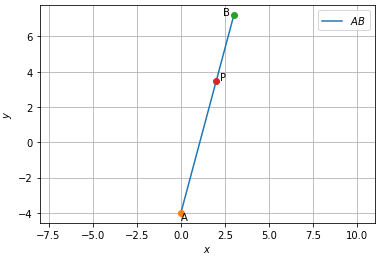
\includegraphics[width=\columnwidth]{solutions/su2021/2/14/Line_Plot_Part2.PNG}
    \caption{Plot of Line $AB$ (Part-2)}
    \label{linform/2/14/Plot of Line $AB$ (Part-2)}
    \end{figure}
\end{enumerate}
\item Construct $PQRS$ where $PQ = 4, QR = 6, RS = 5, PS = 5.5$ and $PR = 7$.
\item Draw $JUMP$ with $JU = 3.5, UM=4, MP = 5, PJ =4.5$ and $PU = 6.5$
\item Construct a quadrilateral $ABCD$ such that $BC=4.5,  AC = 5.5, CD = 5, BD = 7$ and $AD = 5.5$.
\item Can you construct a quadrilateral $PQRS$ with $PQ=3, RS=3, PS=7.5, PR=8$ and $SQ=4$?
\\
\solution 
  
  If we expand the probabilities given further more by substituting the value of x and only considering 0 to 4 hours as the probability of studying in the remaining hours is zero, we get
  
  \begin{table}[ht]
  
 \centering
  
  \begin{tabular}{|c|c|c|c|c|c|}
    \hline
    x &  0 & 1 & 2 & 3 & 4\\
    \hline
    $\Pr\brak{X=x}$ & 0.1& k& 2k & 2k & k\\
    \hline
    
\end{tabular}
\caption{Given probabilities}
\label{Table_1}
\end{table}
we also know that,
\begin{align}
    \sum_{k = 0}^4 \Pr\brak{X = k} = 1 \label{eq 2.0.1}
\end{align}

By substituting the probabilities in \eqref{eq 2.0.1}
\begin{align}
& \implies 0.1 + k + 2k + 2k + k = 1 \\
& \implies 6k = 0.9 \label{eq 2.0.3}
\end{align}

Therefore, from \eqref{eq 2.0.3}
\begin{align}
    k = 0.15
\end{align}
  
 So from \ref{Table_1}
  \begin{table}[ht]
  
  \centering
  \begin{tabular}{|c|c|c|c|c|c|}
    \hline
    x &  0 & 1 & 2 & 3 & 4\\
    \hline
    $\Pr\brak{X=x}$ & 0.1& 0.15& 0.3 & 0.3 & 0.15\\
    \hline
    
\end{tabular} 
\caption{Probabilities after finding k}
\end{table}

\begin{figure}[ht]
    \centering
    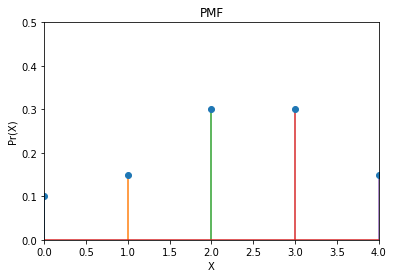
\includegraphics[width=\columnwidth]{solutions/5/28/Figures/PMF.png}
    \caption{Probability Mass Function (PMF)}
    \label{Figure_1}
\end{figure}

We know that, Cumulative Distributive Function (CDF) 
\begin{align}
    F(x) = \Pr\brak{X \le x}
\end{align}

\begin{table}[ht]
  
  \centering
  \begin{tabular}{|c|c|c|c|c|c|}
    \hline
    x &  0 & 1 & 2 & 3 & 4\\
    \hline
    $F(X)$ & 0.1& 0.25& 0.55 & 0.85 & 1\\
    \hline
    
\end{tabular} 
\caption{CDF}
\label{Table_2}
\end{table}

\begin{figure}[ht]
    \centering
    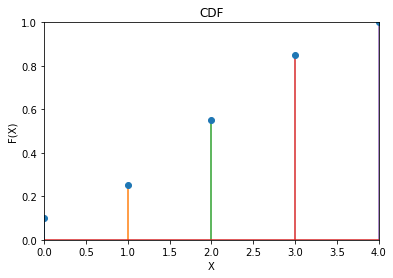
\includegraphics[width=\columnwidth]{solutions/5/28/Figures/CDF.png}
    \caption{Cumulative Distributive Function (CDF)}
    \label{Figure_2}
\end{figure}

And also, 
\begin{align}
     \Pr\brak{x < X \le y} = F\brak{y} - F\brak{x} \label{eq 2.0.6}
\end{align}
         \begin{enumerate}
        \item Probability of studying at least two hours 
           \begin{align}
            & \implies \sum_{k = 2}^4 \Pr\brak{X = k} = \Pr\brak{X \ge 2}\\
            & \implies \Pr\brak{1 < X \le 4} 
        \end{align}
        From \eqref{eq 2.0.6} and \eqref{Table_2}
        \begin{align}
            & = F(4) - F(1)\\
            & = 1 - 0.25\\
            & = 0.75
        \end{align}
        
        \item Probability of studying exactly two hours
        \begin{align}
            & = \Pr\brak{X = 2}\\
            & = 0.3
        \end{align}
        
        \item Probability of studying at most two hours 
        \begin{align}
          & \implies \sum_{k = 0}^2  \Pr\brak{X = k} = \Pr \brak{X \le 2}
         \end{align}
        From \eqref{Table_2}
        \begin{align}
            & = F(2)\\
            & = 0.55
        \end{align}
    \end{enumerate}
  
    \begin{table}[ht]
   
    \centering
  \begin{tabular}{|c|c|c|}
    \hline
    $\Pr\brak{X \geq 2}$ &  $\Pr \brak{X = 2}$ & $\Pr\brak{X \leq 2}$\\
    \hline
     0.75& 0.3& 0.55 \\
    \hline
    Case 1 &Case 2 &Case 3\\
    \hline
\end{tabular} 
 \caption{Final solution}
 \label{Table_3}
\end{table}

\begin{figure}[ht]
    \centering
    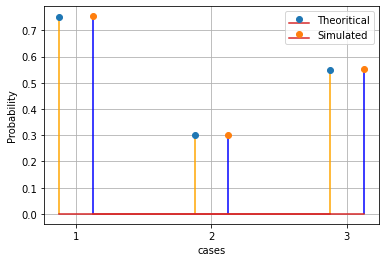
\includegraphics[width=\columnwidth]{solutions/5/28/Figures/stem.png}
    \caption{Simulation and Theoretical Comparison}
    \label{Figure_3}
\end{figure}


\item Construct $LIFT$ such that $LI = 4, IF = 3, TL = 2.5, LF = 4.5, IT=4$.
\item Draw $GOLD$ such that $OL=7.5, GL=6, GD=6, LD = 5, OD = 10$.
\\
\solution 
We obtain the vertices of the rhombus as follows
\begin{align}
\vec{A} = \myvec{-3\\0},
\vec{B} = \myvec{0\\-3.5},
\vec{C} = \myvec{3\\0},
\vec{D} = \myvec{0\\3.5}
\end{align}
which are plotted in Fig. \ref{quad/45/fig:Rhombus ABCD}.
%
\begin{figure}[ht!]
\centering
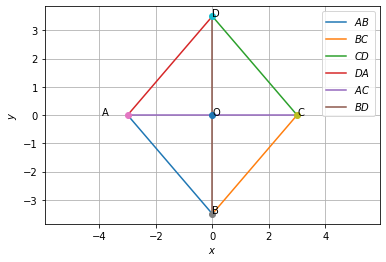
\includegraphics[width=\columnwidth]{solutions/quad/45/figure2.png}
\caption{Rhombus ABCD}
\label{quad/45/fig:Rhombus ABCD}
\end{figure}


\item DRAW rhombus $BEND$ such that $BN = 5.6$, $DE = 6.5$.
\item construct a quadrilateral MIST where $MI = 3.5, IS = 6.5, \angle M = 75 \degree, \angle I = 105 \degree$ and $\angle S = 120 \degree$.
\item Can you construct the above quadrilateral MIST if $\angle M = 100 \degree$ instead of $75 \degree$.
\item Can you constrcut the quadrilateral PLAN if $PL = 6, LA = 9.5, \angle P = 75 \degree, \angle L = 150 \degree$ and $\angle A = 140 \degree$?
\item Construct $MORE$ where $MO = 6, OR = 4.5, \angle M = 60 \degree, \angle O = 105 \degree, \angle R = 105 \degree$.
\item Construct $PLAN$ where $PL = 4, LA = 6.5, \angle P = 90 \degree, \angle A = 110\degree$ and $\angle N = 85\degree$.
\item Draw  rectangle $OKAY$ with $OK = 7$ and $KA = 5$.
\item Construct $ABCD $, where $AB = 4, BC = 5, Cd = 6.5, \angle B = 105 \degree$ and $\angle C = 80\degree$.
\\
\solution 

Let 
    \begin{align}
    &\angle B= 105\degree=\theta \label{quad/42/eq1}
    \\
    &\angle C= 80\degree=\alpha \label{quad/42/eq2}
    \\
    &\norm{\vec{A}-\vec{B}} =4=p \label{quad/42/eq3}
    \\
    &\norm{\vec{C}-\vec{B}} =5=q \label{quad/42/eq4}
    \\
     &\norm{\vec{D}-\vec{C}} =6.5=r \label{quad/42/eq5}
    \end{align}
and 
\begin{align}
    &\vec{B}=\myvec{0\\0}, \vec{C}=\myvec{5\\0}
\end{align}

\begin{lemma}
\label{quad/42/lemma}
\begin{align}
  & \vec{A} = p \vec{b}  \quad \brak{\because \vec{B}=\myvec{0\\0}} \label{quad/42/eq a}
\\
  & \vec{D} =\vec{C} + r \vec{c} \label{quad/42/eq b}
\end{align}
where 
\begin{align}
 \vec{b} = \myvec{\cos B \\ \sin B } ,\vec{c} = \myvec{\cos C\\ \sin C }
\end{align}
\end{lemma}
Thus, 
\begin{align}
 \vec{A} &=4\myvec{\cos 105 \\\sin 105 }
\\
&=\myvec{-1.03\\3.86}
\end{align}
and 
\begin{align}
\vec{D} &=\myvec{5\\0} + 6.5\myvec{\cos 80 \\\sin 80 }
\\
&=\myvec{6.12\\6.39}
\end{align}
which are then used to plot Fig. \ref{quad/42/fig:Quadrilateral ABCD}	
\begin{figure}[!ht]
\centering
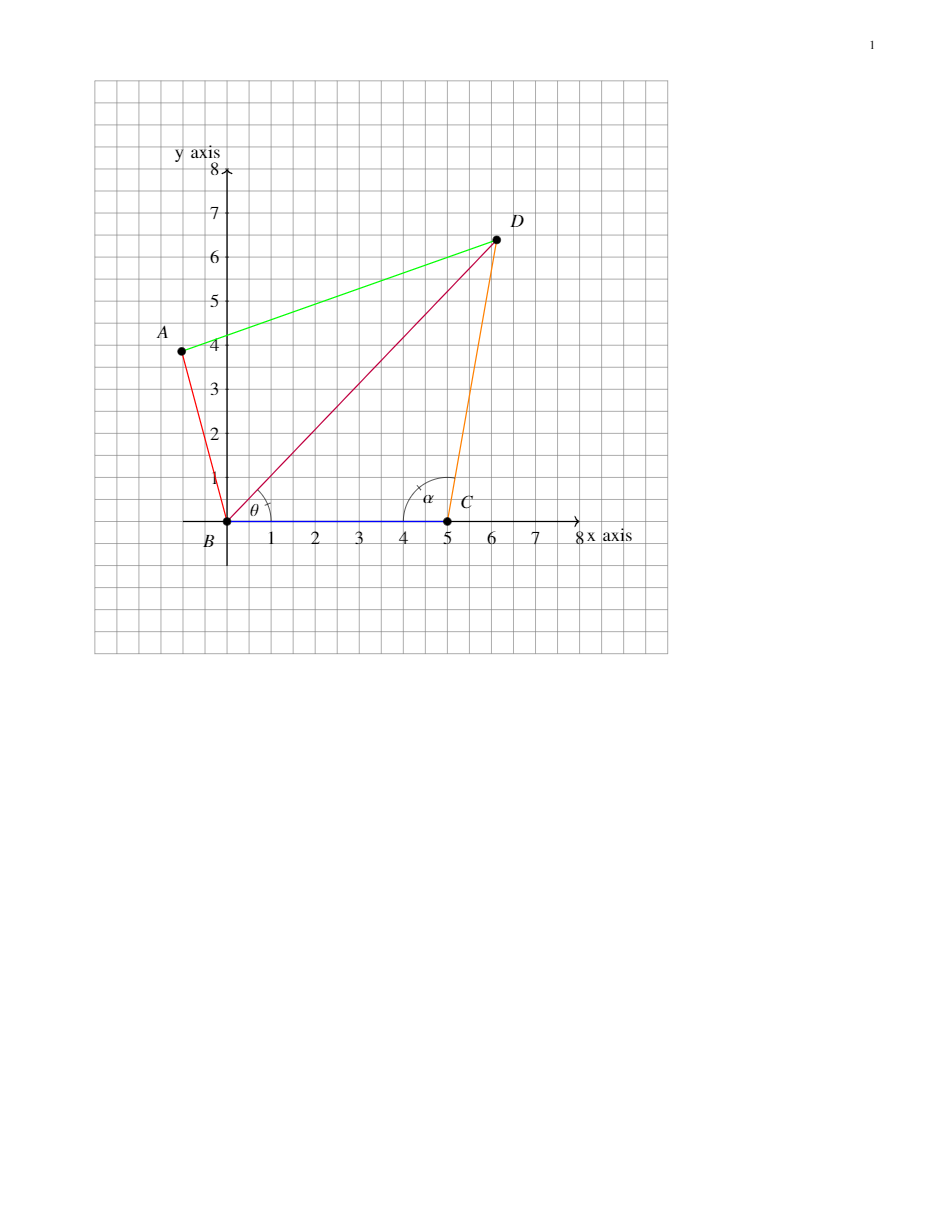
\includegraphics[ width=\columnwidth]{solutions/quad/42/FIGURE.png}
\caption{Quadrilateral ABCD}
\label{quad/42/fig:Quadrilateral ABCD}	
\end{figure}

%
\item Construct $DEAR$ with $DE = 4, EA = 5, AR = 4.5, \angle E = 60 \degree$ and $\angle A = 90 \degree$.
\\
\solution 
We obtain the vertices of the rhombus as follows
\begin{align}
\vec{A} = \myvec{-3\\0},
\vec{B} = \myvec{0\\-3.5},
\vec{C} = \myvec{3\\0},
\vec{D} = \myvec{0\\3.5}
\end{align}
which are plotted in Fig. \ref{quad/45/fig:Rhombus ABCD}.
%
\begin{figure}[ht!]
\centering
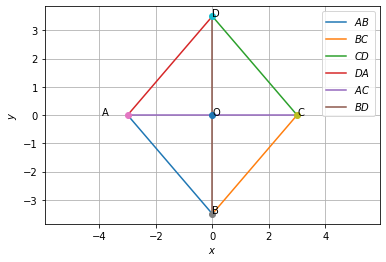
\includegraphics[width=\columnwidth]{solutions/quad/45/figure2.png}
\caption{Rhombus ABCD}
\label{quad/45/fig:Rhombus ABCD}
\end{figure}


\item Construct $TRUE$ with $TR = 3.5, RU = 3, UE = 4 \angle R = 75\degree$ and $\angle U = 120\degree$.
\\
\solution 
We obtain the vertices of the rhombus as follows
\begin{align}
\vec{A} = \myvec{-3\\0},
\vec{B} = \myvec{0\\-3.5},
\vec{C} = \myvec{3\\0},
\vec{D} = \myvec{0\\3.5}
\end{align}
which are plotted in Fig. \ref{quad/45/fig:Rhombus ABCD}.
%
\begin{figure}[ht!]
\centering
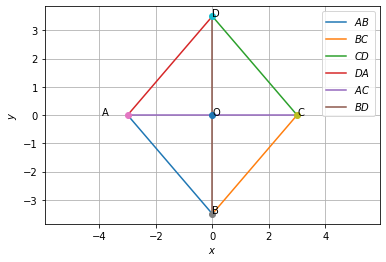
\includegraphics[width=\columnwidth]{solutions/quad/45/figure2.png}
\caption{Rhombus ABCD}
\label{quad/45/fig:Rhombus ABCD}
\end{figure}




\item Can you construct a rhombus $ABCD$ with $AC = 6$ and $BD = 7$?
\item Draw a square $READ$ with $RE = 5.1$.
\\
\solution 
The centers and radii of the two circles without any loss of generality are given in Table \ref{constr/55/tab:table1}
%
\begin{table}[!ht]
\begin{center}
\begin{tabular}{ | m{2cm} | m{2cm} | m{2cm} |} 
\hline
 & Circle 1 & Circle 2 \\
\hline
Centre  & $\vec{A}$=\myvec{0\\0} & $\vec{B}$=\myvec{3\\0} \\ 
\hline
Radius & $r_{1}=r_{2}=3$  \\ 
\hline
\end{tabular}
\end{center}
\caption{Input values}
\label{constr/55/tab:table1}

\end{table}

% The choice for $\vec{A}$ and $\vec{B}$ is valid as:
% \begin{align}
% \norm{\vec{B}-\vec{A}} = \norm{\vec{A}-\vec{B}}=\norm{\vec{B}}  = 3 \quad \brak{\because \vec{A}=0}
% \end{align}

Let 
\begin{align}
\vec{u}=\myvec{\cos \theta\\  \sin \theta},  \theta \in \sbrak{0,2\pi}.
\end{align}

Then on Circle 1  and Circle 2 are  given by 
\begin{align}
\vec{x}&=\vec{A}+r\vec{u}
\\
\vec{x}&=\vec{B}+r\vec{u}
\end{align}

Fig. \ref{constr/55/fig:circle} is plotted using the above equations.
%
\begin{figure}[!ht]
\centering
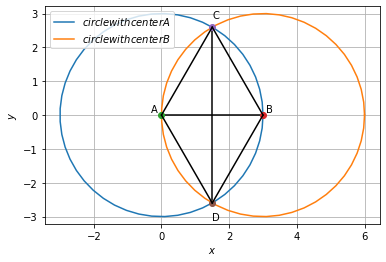
\includegraphics[width=\columnwidth]{solutions/55/Figures/figure3.png}
\caption{Circles with their points of intersection}
\label{constr/55/fig:circle}	
\end{figure}
Fig. \ref{constr/55/fig:circle} 

The general equation of Circle 1 is given by 
\begin{align}
    \norm{\vec{x}-\vec{A}}^2 &= r^2
    \\
\vec{x}^{\top}\vec{x} - 2\vec{A}^{\top}\vec{x} + \norm{\vec{A}}^2 -r_{1}^2 &= 0\label{constr/55/eq:14}
\end{align}
Similarly, for Circle 2,
\begin{align}
\vec{x}^{\top}\vec{x} - 2\vec{B}^{\top}\vec{x} + \norm{\vec{B}}^2 -r_{2}^2 = 0\label{constr/55/eq:15}
\end{align}
Subtracting \eqref{constr/55/eq:15} from \eqref{constr/55/eq:14},
\begin{align}
2\vec{B}^{\top}\vec{x}=\norm{\vec{B}}^2
\\
\myvec{1&0}\vec{x}=\frac{3}{2}
\end{align}
which can be expressed as
\begin{align}
\vec{x} &=\frac{1}{2}\myvec{3\\ 0} + \lambda \myvec{0\\1}\label{constr/55/eq:19}\\
&=\vec{q}+\lambda\vec{m} \text{ where}\label{constr/55/eq:20}\\
\vec{q}&=\myvec{1.5\\ 0},
\vec{m}=\myvec{0\\1}
\end{align}
Substituting \eqref{constr/55/eq:20} in \eqref{constr/55/eq:14}
\begin{align}
\norm{\vec{x}}^2=r^2\quad \brak{\because \vec{A}=0}
\\
\norm{\vec{q}+\lambda\vec{m}}^2=r^2\\
(\vec{q}+\lambda \vec{m})^{\top}(\vec{q}+\lambda \vec{m})=r^2\\
\implies \vec{q}^{\top}(\vec{q}+\lambda \vec{m})+\lambda \vec{m}^{\top}(\vec{q}+\lambda \vec{m})=r^2
\\
\implies \norm{\vec{q}}^2+\lambda\vec{q}^{\top}\vec{m}+\lambda\vec{m}^{\top}\vec{q}+\lambda^2\norm{\vec{m}}^2=r^2
\\
\implies \norm{\vec{q}}^2+2\lambda\vec{q}^{\top}\vec{m}+\lambda^2\norm{\vec{m}}^2=r^2 
% \\
% \implies \lambda(\lambda\norm{\vec{m}}^2+2\vec{q}^{\top}\vec{m})=r^2-\norm{\vec{q}}^2\\
% \implies\lambda^2\norm{\vec{m}}^2=9-\norm{\vec{q}}^2
\\
\implies \lambda=\pm \sqrt{\frac{9-\norm{\vec{q}}^2}{\norm{\vec{m}}^2}} \quad \because \vec{q}^{\top}\vec{m} = 0
% \lambda^2=6.75\\
% \lambda=+\sqrt{6.75},-\sqrt{6.75}
\end{align}
Substituting the value of $\lambda$ in \eqref{constr/55/eq:20},
\begin{align}
%\vec{x}=\vec{q}+\lambda\vec{m}\\
\vec{C}&=\vec{q}+\lambda\vec{m}\\
\vec{D}&=\vec{q}-\lambda\vec{m} \\
\implies (\vec{A}-\vec{B})^{\top}(\vec{C}-\vec{D})
&=2\myvec{-3&0}\myvec{0\\\sqrt{6.75}}
\\
&=0
\\
\implies AB\perp CD
\end{align}


% We have $\vec{C}$ and $\vec{D}$ as points of intersection and $r_{1}=r_{2}$.So,
% \begin{align}
% \norm{\vec{C}-\vec{A}}^2 = \norm{\vec{C}-\vec{B}}^2
% \end{align}
% \begin{align}
% \implies(\vec{C}-\vec{A})^{\top}(\vec{C}-\vec{A})=(\vec{C}-\vec{B})^{\top}(\vec{C}-\vec{B})
% \\
% \implies \vec{A}^{\top}\vec{C}-\vec{B}^{\top}\vec{C}=\vec{C}^{\top}\vec{B}-\vec{C}^{\top}\vec{A}+\norm{\vec{A}}^2-\norm{\vec{B}}^2 
% \end{align}
% \begin{align}
% \implies2\times \vec{A}^{\top}\vec{C}-2\times\vec{B}^{\top}\vec{C}=\norm{\vec{A}}^2-\norm{\vec{B}}^2 \label{constr/55/eq:1}
% \end{align}
% Similarly,using:
% \begin{align}
% \norm{\vec{D}-\vec{A}}^2 = \norm{\vec{D}-\vec{B}}^2
% \end{align}
% We get:
% \begin{align}
% 2\times \vec{A}^{\top}\vec{D}-2\times\vec{B}^{\top}\vec{D}=\norm{\vec{A}}^2-\norm{\vec{B}}^2 \label{constr/55/eq:2}
% \end{align}

% Subtracting equation \ref{constr/55/eq:2} from equation \ref{constr/55/eq:1}:
% \begin{align}
% 2\times(\vec{A}^{\top}-\vec{B}^{\top})(\vec{C}-\vec{D})=0
% \\
% \implies (\vec{A}-\vec{B})^{\top}(\vec{C}-\vec{D})=0
% \\
% \implies AB\perp CD
% \end{align}

\item Draw a rhombus who diagonals are $5.2$ and $6.4$.
\item Draw a rectangle with adjacent sides $5$ and $4$.
\\
\solution 
We obtain the vertices of the rhombus as follows
\begin{align}
\vec{A} = \myvec{-3\\0},
\vec{B} = \myvec{0\\-3.5},
\vec{C} = \myvec{3\\0},
\vec{D} = \myvec{0\\3.5}
\end{align}
which are plotted in Fig. \ref{quad/45/fig:Rhombus ABCD}.
%
\begin{figure}[ht!]
\centering
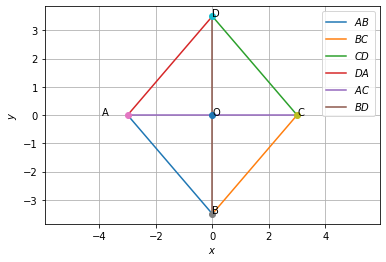
\includegraphics[width=\columnwidth]{solutions/quad/45/figure2.png}
\caption{Rhombus ABCD}
\label{quad/45/fig:Rhombus ABCD}
\end{figure}


\item Draw a parallelogram $OKAY$ with $OK = 5.5$ and $KA = 4.2$.
\\
\solution  There are infinite number of parallelograms that can be draw.  For a unique parallelogram, one angle
needs to be specified.

\item Construct a kite $EASY$ if $AY = 8, EY = 4$ and $SY = 6$.


%\end{enumerate}
%
